\documentclass{standalone}
\usepackage[dvipsnames]{xcolor}
\usepackage{tikz}
\usetikzlibrary{patterns,decorations.markings}

\tikzstyle{v par}=              [dash pattern=on 10pt off 5pt,color=red,line width = 2pt]
\tikzstyle{z direction}=      [dash pattern=on 10pt off 5pt on 2pt off 5pt, color=Blue,line width = 2pt]

\begin{document}
 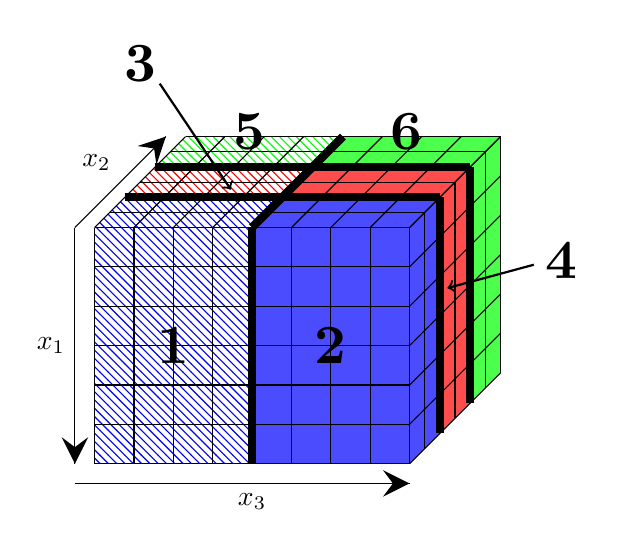
\begin{tikzpicture}[scale=0.5]
  \def\nx{8}
\def\ny{6}
\def\nz{6}

\tikzset{myptr/.style={decoration={markings,mark=at position 1 with %
    {\arrow[scale=3,>=stealth]{>}}},postaction={decorate}}}

\fill[pattern=north west lines, pattern color=blue] (0,0,0) -- (\nx/2,0,0) -- (\nx/2,-\ny,0) -- (0,-\ny,0) -- (0,0,0);
\fill[pattern=north west lines, pattern color=blue] (0,0,0) -- (\nx/2,0,0) -- (\nx/2,0,-\nz/3) -- (0,0,-\nz/3) -- (0,0,0);
\fill[blue!70] (\nx/2,0,0) -- (\nx,0,0) -- (\nx,-\ny,0) -- (\nx/2,-\ny,0) -- (\nx/2,0,0);
\fill[blue!70] (\nx/2,0,0) -- (\nx,0,0) -- (\nx,0,-\nz/3) -- (\nx/2,0,-\nz/3) -- (\nx/2,0,0);
\fill[blue!70] (\nx,0,0) -- (\nx,-\ny,0) -- (\nx,-\ny,-\nz/3) -- (\nx,0,-\nz/3) -- (\nx,0,0);

\fill[pattern=north west lines, pattern color=red] (0,0,-\nz/3) -- (\nx/2,0,-\nz/3) -- (\nx/2,0,-2*\nz/3) -- (0,0,-2*\nz/3) -- (0,0,-\nz/3);
\fill[red!70] (\nx/2,0,-\nz/3) -- (\nx,0,-\nz/3) -- (\nx,0,-2*\nz/3) -- (\nx/2,0,-2*\nz/3) -- (\nx/2,0,-\nz/3);
\fill[red!70] (\nx,0,-\nz/3) -- (\nx,-\ny,-\nz/3) -- (\nx,-\ny,-\nz*2/3) -- (\nx,0,-\nz*2/3) -- (\nx,0,-\nz/3);

\fill[pattern=north west lines, pattern color=green] (0,0,-2*\nz/3) -- (\nx/2,0,-\nz*2/3) -- (\nx/2,0,-\nz) -- (0,0,-\nz) -- (0,0,-2*\nz/3);
\fill[green!70] (\nx/2,0,-\nz*2/3) -- (\nx,0,-\nz*2/3) -- (\nx,0,-\nz) -- (\nx/2,0,-\nz) -- (\nx/2,0,-\nz*2/3);
\fill[green!70] (\nx,0,-\nz*2/3) -- (\nx,-\ny,-\nz*2/3) -- (\nx,-\ny,-\nz) -- (\nx,0,-\nz) -- (\nx,0,-\nz*2/3);

\foreach \y in{0,...,\ny}
{
    \draw (0,-\y ,0) -- (\nx,-\y ,0);
    \draw (\nx,-\y ,-\nz) -- (\nx,-\y ,0);
}
\foreach \x in{0,...,\nx}
{
    \draw (\x ,0,0) -- (\x ,-\ny,0);
    \draw (\x ,0,-\nz) -- (\x ,0,0);
}

\foreach \z in {0,...,\nz}
{
   \draw (\nx,0,-\z ) -- (\nx,-\ny,-\z );
   \draw (0,0,-\z ) -- (\nx,0,-\z );
}

\pgfmathsetmacro\nxMax{\nx-1}
 \pgfmathsetmacro\nyMax{\ny-1}
 \pgfmathsetmacro\nzMax{\nz-1}
 
 \pgfmathsetmacro\nySplitMax{\ny/3-1}
 \pgfmathsetmacro\nzSplitMax{\nz/2-1}
 
 
 \draw[line width=3pt] (0,0,-\nz*2/3) -- (\nx,0,-\nz*2/3);
 \draw[line width=3pt] (\nx,0,-\nz*2/3) -- (\nx,-\ny,-\nz*2/3);
 \draw[line width=3pt] (0,0,-\nz/3) -- (\nx,0,-\ny/3);
 \draw[line width=3pt] (\nx,0,-\nz/3) -- (\nx,-\ny,-\nz/3);
 \draw[line width=3pt] (\nx/2,0,0) -- (\nx/2,0,-\nz);
 \draw[line width=3pt] (\nx/2,0,0) -- (\nx/2,-\ny,0);

\node[scale=2] at (\nx/4,-\ny/2,0) {\bf 1};
\draw[->,thick] (0.5,2.5,-3) -- (2.5,0,-2.5);
\node[scale=2] at (0,3,-\nz*3/6) {\bf 3};
\node[scale=2] at (\nx/4,0.5,-\nz*5/6) {\bf 5};
\node[scale=2] at (\nx*3/4,-\ny/2,0) {\bf 2};
\draw[<-,thick] (\nx,-2.5,-2.5) -- (\nx+2,-2.1,-\nz/2);
\node[scale=2,right] at (\nx+1.8,-2,-\nz/2) {\bf 4};
\node[scale=2] at (\nx*3/4,0.5,-\nz*5/6) {\bf 6};

\draw[myptr] (-.5,0,0) -- (-.5,-\ny,0);
\node[left] at (-.5,-\ny/2,0) {$x_1$};

\draw[myptr] (-.5,0,0) -- (-.5,0,-\nz);
\node[left] at (-.5,.5,-\nz/2) {$x_2$};

\draw[myptr] (-.5,-\ny-.5,0) -- (\nx,-\ny-.5,0);
\node[below] at (\nx/2,-\ny-.5,0) {$x_3$};
 \end{tikzpicture}
\end{document}
